%----------------------------------------------------------------------------------------
%	PACKAGES AND DOCUMENT CONFIGURATIONS
%----------------------------------------------------------------------------------------

\documentclass[11pt,a4paper]{article}

\usepackage{graphicx} % Required for the inclusion of images
\usepackage{natbib} % Required to change bibliography style to APA
\usepackage{amsmath} % Required for some math elements 
\usepackage{subcaption}
\usepackage{pbox}
\usepackage{listings}
\usepackage{longtable}
\usepackage[justification=centering]{caption}
\usepackage[nomarkers,nofiglist,notablist]{endfloat}
\DeclareDelayedFloatFlavor*{longtable}{table}
\usepackage[margin=0.9in]{geometry}
\usepackage{sectsty}
\sectionfont{\fontsize{12}{15}\selectfont}
\setlength\parindent{0pt} % Removes all indentation from paragraphs
\usepackage{todonotes}
\usepackage{units} % for nice fractions \nicefrac{}{}
\usepackage[hidelinks=true]{hyperref}
\def\labelitemi{--}

\renewcommand{\labelenumi}{\alph{enumi}.} % Make numbering in the enumerate environment by letter rather than number

%%%%%%%%%% Start TeXmacs macros
\newcommand{\nocomma}{}
\newcommand{\noplus}{}
\newcommand{\tmop}[1]{\ensuremath{\operatorname{#1}}}
\newcommand{\upl}{+}
%%%%%%%%%% End TeXmacs macros

%----------------------------------------------------------------------------------------
%	DOCUMENT INFORMATION
%----------------------------------------------------------------------------------------

\title{\vspace{-2cm}Machine Translation Assignment 3: Reranking\vspace{-2cm}} % Title

%\author{s0907677, s1112290} % Author name

\date{}

\begin{document}

\maketitle % Insert the title, author and date

\section*{Q1}


Since we are using argmax over the sum of weighted features to find the best translation, changing the sign on one feature weight means that we are looking for its minimum, rather than maximum, value. If the weight of language model log likelihood is set to -1, we can expect the chosen translation to not be a particularly fluent English sentence.
\section*{Q2}
When local reordering is allowed, the search space expands, since at each step we need to consider three possible sources of the next part of the English translation:
\begin{itemize}
	\item the next French phrase (as was always the case in the monotone decoder);
	\item the second next French phrase;
	\item the previous French phrase.
\end{itemize}
The latter two cases account for the fact that hypotheses might be created by skipping one French phrase and translating a next one. If that was the way a hypothesis was generated, the only way of extending it is to go back and translate the skipped part.

Instead of modelling explicitly these three possibilities, we decided to describe the search space more succinctly by positing that there is only one possible way of expanding a hypothesis, namely finding next two phrases and swapping them. This reformulation is possible thanks to the introduction of an artificial empty phrase, which we call the $\varepsilon$ phrase.

In recursive terms, given the last word in the translation, \textit{e}, and the index of the last translated French word, \textit{j}, we are looking for such pair of indices \textit{i, c} that:
\begin{itemize}
	\item $i < c \leq j$
	\item translation of French[\textit{i,c}] ends in word \textit{e}
	\item translation of French[\textit{c,j}] proceeds translation of French[\textit{i,c}] in the English sentence
	\item the translation and language model probability is maximized
\end{itemize}
Given that French[\textit{c,j}] might be the $\varepsilon$ phrase, this formulation also covers the no-reordering case.
\vspace{4mm} %4mm vertical space

Our full definition of $h(j,e)$ is specified as follows:
\vspace{4mm} %4mm vertical space


\input{figures/h.tex}

\section*{Q3}
Table~\ref{BLEUtable} and figure~\ref{BLEU} illustrate the BLEU scores achieved by rerankers using a variety of feature combinations.

\begin{figure}
	\centering
	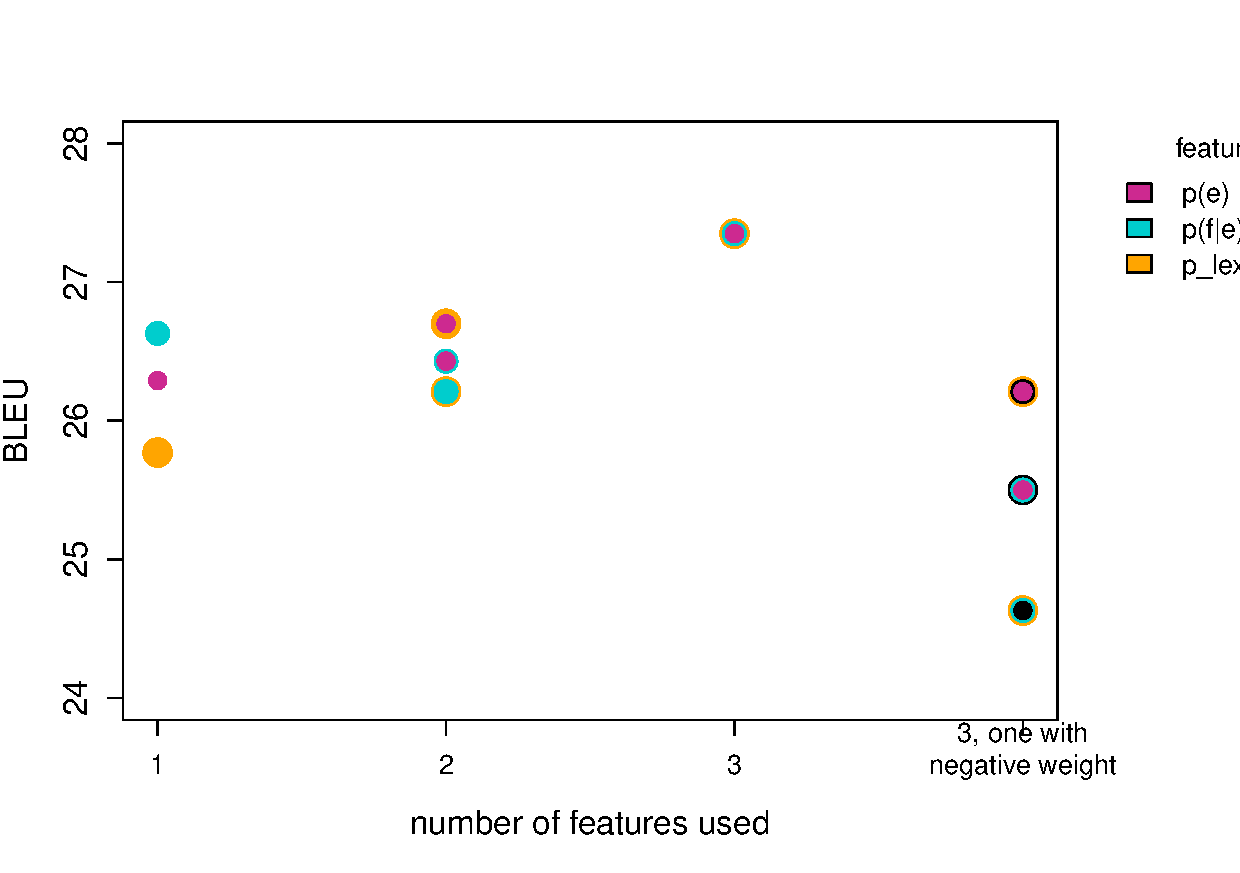
\includegraphics[scale=.75]{figures/q3.pdf}
	\caption{BLEU score as dependent on candidate translation features used for reranking.}\label{BLEU}
\end{figure}

\begin{table}
	\centering
	\begin{tabular}{||c|c|c|c||}
		\hline
		\textbf{p(e)} & \textbf{p(f$|$e)} & \textbf{p\_lex(e$|$f)} & \textbf{BLEU}\\
		\hline
		1&1&1&27.35\\
		\hline
		\multicolumn{4}{||c||}{manipulating p(e)}\\
		\hline
		1&0&0&26.29\\
		0&1&1&26.21\\
		-1&1&1&24.63\\
		-1&0&0&24.19\\
		\hline
		\multicolumn{4}{||c||}{manipulating p(f$|$e)}\\
		\hline
		0&1&0&26.63\\
		1&0&1&26.70\\
		1&-1&1&26.21\\
		0&-1&0&25.58\\
		\hline
		\multicolumn{4}{||c||}{manipulating p\_lex(e$|$f)}\\
		\hline
		0&0&1&25.77\\
		1&1&0&26.43\\
		1&1&-1&25.50\\
		0&0&-1&24.84\\
		\hline
		\end{tabular}
		\caption{BLUE scores achieved with different combinations of feature weights.}\label{BLEUtable}
\end{table}

The first thing to note is that the best BLEU score model is achieved when all three features are used, which suggests that all of them contribute useful information.

The influence of particular features on the BLEU score is quite opaque. There is no single most informative feature. The best one to use in isolation is p(f$|$e); the largest BLEU decrease is observed when p(e) is eliminated or reversed. Interestingly, combining TM likelihood with one other feature has a negative influence on the score, but combining it with both brings the score to maximum.  

\section*{Q4}

The oracle translations tend to have better BLEU scores. The oracle outputs are intuitively better, but not without exceptions. Let's look at the first example in section \textit{Oracle} of table~\ref{translation_compare}.
  
The oracle translation, on top of from not omitting \textit{the residents}, accounts for the English distinction between \textit{house} and \textit{home}. However, the preferred preposition of \textit{the stairwell} was correctly chosen by the default reranker and not by the oracle.
Similarly in the second and third example, the oracle provides a more fluent translation, being able to create a fully formed sentence made up of complex clause types.

However, there are still many less-than-good translations. These occur inter alia when sentences have rare special characters (example five); Russian conventions for comparatives are retained, resulting in poorly-formed English sentences (example six); sentence is longer, with more complex clausal structure is (example seven).

Since the oracle's aim it to maximize BLEU by choosing from the provided top candidates, the above shortcomings likely reflect both the deficiencies of the decoder (and statistical models) used to produce the candidates and of BLEU as a metric of translation quality. Sometimes there are no good translations among the candidates, as for the sentence about 20 planes. In other cases, illustrated by example four in table~\ref{translation_compare}, even though the choice of the default reranker is clearly better, its BLUE score is lower.

%\begin{longtable}
%	\centering
	\begin{longtable}{||c|c||}
	\hline
	\textbf{Default} & \textbf{Flipped LM}\\
	\hline
	\parbox{7cm}{\vspace{.5\baselineskip} "cold and inhuman": anders беринг\\breivik first publicly trial\vspace{.5\baselineskip}} &
	\parbox{7cm}{\vspace{.5\baselineskip} "cold and inhuman": anders fogh\\беринг breivik publicly appears before\\by the court for the first time"\vspace{.5\baselineskip}}\\
	\hline
	\parbox{7cm}{\vspace{.5\baselineskip} after the summer the researchers\\wanted to learn more about\\these people.\vspace{.5\baselineskip}} &
	\parbox{7cm}{\vspace{.5\baselineskip} after summer of the tragedy\\the researchers want to learn\\more about the these people.\vspace{.5\baselineskip}}\\
	\hline
	\parbox{7cm}{\vspace{.5\baselineskip} someone can use the ' language '\\when answering a question :\\" well... the truth... how do i know...\\as far as i know."\vspace{.5\baselineskip}} &
	\parbox{7cm}{\vspace{.5\baselineskip} somebody can use the ' qualification\\language ', when responds to\\a difficult question :" well...\\the truth... as far as i know...\\as far as i know."\vspace{.5\baselineskip}}\\
	\hline
	\parbox{7cm}{\vspace{.5\baselineskip} " this paper tiger, the army barracks,\\buildings and bombs without enough\\trained soldiers, to accomplish the\\mission," panetta said in his introductory\\remarks at the pentagon.\vspace{.5\baselineskip}}&
	\parbox{7cm}{\vspace{.5\baselineskip} "it 's a paper tiger, the army with the\\barracks, buildings and bombs without\\enough trained soldiers, who can\\accomplish the mission,"panetta said in\\ their introductory remarks in the pentagon.\vspace{.5\baselineskip}}\\
	\hline
	\parbox{7cm}{\vspace{.5\baselineskip} you need to keep in mind 5,000\\these concepts, ideas - them all together.\vspace{.5\baselineskip}}&
	\parbox{7cm}{\vspace{.5\baselineskip} you need to keep in the head\\of the 5,000 of ideas - these concepts,\\combining them all together...\vspace{.5\baselineskip}}\\
	\hline
	\textbf{Default} & \textbf{Oracle}\\
	\hline
	\parbox{7cm}{\vspace{.5\baselineskip} the police statement reported that\\the home noticed smoke in\\the apartment stairwell and... \vspace{.5\baselineskip}} &
	\parbox{7cm}{\vspace{.5\baselineskip} police in a statement reported that\\residents of the house noticed\\smoke on the apartment stairwell and... \vspace{.5\baselineskip}}\\
	\hline
	\parbox{7cm}{\vspace{.5\baselineskip} bella in the fourth finally able\\to marry her lover\vspace{.5\baselineskip}}&
	\parbox{7cm}{\vspace{.5\baselineskip} bella in a fourth part finally\\manages to marry her beloved.\vspace{.5\baselineskip}}\\
	\hline
	\parbox{7cm}{\vspace{.5\baselineskip} before, if you want to interview\\people from the british national party,\\would be very difficult to\vspace{.5\baselineskip}} &
	\parbox{7cm}{\vspace{.5\baselineskip} previously, if you wanted to interview\\people from the british national party,\\it would be very difficult\vspace{.5\baselineskip}}\\
	\hline
	\parbox{7cm}{\vspace{.5\baselineskip} two 19 - year - old tried to help\\young people, but were\\immediately beaten by four men. \vspace{.5\baselineskip}}&
	\parbox{7cm}{\vspace{.5\baselineskip} two 19 - year - olds young people\\trying to help, but were\\just beaten by the four men. \vspace{.5\baselineskip}}\\
	\hline
	 & \parbox{7cm}{\vspace{.5\baselineskip}including an option to buy 20 more\\planes, total volume, in fact,\\the \$26 billion.\vspace{.5\baselineskip}}\\
	 \hline
	 & \parbox{7cm}{\vspace{.5\baselineskip}but residents complaining of the dirt\\and noise, in many communities\\is becoming more and more.\vspace{.5\baselineskip}}\\
	 \hline
	 & \parbox{7cm}{\vspace{.5\baselineskip}all four birds used the wire to make\\and used hooks hooks, to\\a bucket for pen and pull\\him out of the cylinder\vspace{.5\baselineskip}}\\
	\hline
	\textbf{Deafult} & \textbf{Best parameters}\\
	\hline
	\parbox{7cm}{\vspace{.5\baselineskip} the training took place late on\\monday on...\vspace{.5\baselineskip}}&
	\parbox{7cm}{\vspace{.5\baselineskip} the latest training took place late\\on monday on...\vspace{.5\baselineskip}}\\
	\hline
	\parbox{7cm}{\vspace{.5\baselineskip} will new measures supported the council\\on foreign affairs or расколют lawmakers\\as the june bill ?...\vspace{.5\baselineskip}}&
	\parbox{7cm}{\vspace{.5\baselineskip} whether the new measures will receive full\\support of the council on foreign affairs\\or расколют legis...\vspace{.5\baselineskip}}\\
	\hline
	\parbox{7cm}{\vspace{.5\baselineskip} facebook also draws all kinds of data\\about its users. \vspace{.5\baselineskip}}&
	\parbox{7cm}{\vspace{.5\baselineskip} facebook also constantly pulls all sorts\\of data about its users.\vspace{.5\baselineskip}}\\
	\hline
	\caption{Comparison of outputs of the reranker with different configurations.}\label{translation_compare}
	\end{longtable}
	%\caption{Comparison of outputs of the reranker with different configurations.}\label{translation_compare}
%\end{longtable}

\section*{Q5}

A grid search through all the three features (with weights between -5 and 5) was carried out. The highest BLEU score (28.16, 0.81 higher than default) was achieved with the following configuration of feature weights:

\centerline{p(e) : 2,    p(e$|$f) : 3,    p\_lex(f$|$e) : 5}

Qualitatively, the translations chosen with the optimal parameter configuration are generally of better fluency and accuracy. They are also more verbose, which is a good thing, given the tendency of the default model to favour too short sentences. Limiting the relative weight of the p(e) lets the intended Russian meaning to be preserved. This is seen in the first example in section \textit{Best parameters} in table~\ref{translation_compare}, where the default reranker drops the adverb \textit{latest}.

The second example shows how a more precise translation is created as a more fluent syntax is produced by allowing larger but less frequent clause types.
   
In many cases default and optimal reranker output differ in one choice between synonymous words or phrases. Sometimes the default reranker picks a better synonym, as in the final example in table~\ref{translation_compare}. Potentially the heavy weighting of p(e$|$f) and p\_lex(f$|$e) encourages a closer match to original Russian, at a cost of choosing a word less appropriate in the English context.
\section*{Q6}

Similarly to the non-reordering decoder, increases in the number of
translations $k$ lead to major improvements at first, but fewer improvements
$k>50$. In contrast to the results obtained from the simple decoder,
increases in the stack size $s$ do not fade out as quickly. The changes also
have a larger effect for smaller $s$, with the biggest difference between
$s=1$ and $s=2$. Even in the reordering decoder, we do not observe any
performance increases for $s>20$.

We note that $k$ and $s$ have a much larger effect on runtime than they have
for the simple decoder. Nonetheless, the run times of both decoders are in
the same order of magnitude (see Fig.~\ref{swaptime}). For $k = s = 10$, the
sentences are relatively well-formed, though still difficult to understand.
Since we are still using a bigram model, it is not surprising that long-term
dependencies are not correctly resolved.

\begin{figure}
	\centering
	\begin{subfigure}{.8\linewidth}
		\includegraphics[scale=.65]{figures/d2_k.pdf}
		\caption{Increasing maximum number of translations, range [1--100].}
	\end{subfigure}
	\hskip2em
	\begin{subfigure}{.8\linewidth}
		\includegraphics[scale=.65]{figures/d2_s.pdf}
		\caption{Increasing stack size, range [1--100].}
	\end{subfigure}
    \caption{Performance of decoder with local reordering.}\label{swap}
\end{figure}

\begin{figure}
	\centering
	\begin{subfigure}{.45\linewidth}
		\includegraphics[scale=.35]{figures/time.pdf}
		\caption{Decoding time as function of maximum number of translations.}
	\end{subfigure}
	\hskip2em
	\begin{subfigure}{.45\linewidth}
		\includegraphics[scale=.35]{figures/time_d1_d2.pdf}
		\caption{Decoding time as a function of stack size.}
	\end{subfigure}
	\caption{Decoding time for the three decoders.}\label{swaptime}
\end{figure}


\section*{Q7}
We decided to implement the Minimum Error Training Rate algorithm for choosing optimal model parameter values, described in \cite{och2003}. The aim of weight tuning is to make the best translations achieve the highest model scores. In this assignment we use BLEU as the measure of translation goodness. While with only 4 features hand-tuning is feasible, in principle the number could be much larger, requiring a principled method of searching through the parameter space. We apply MERT to learn the optimal weights of p(e), p(e$|$f), p\_lex(f$|$e), and len features from the training data. These weights are supplied to the reranker for use on the test data.

For the MERT algorithm itself two variables are important: the stopping criterion and initial parameter values. We stop when improvement in BLEU from previous iteration is less than 0.0001. We start at a point whose coordinates are randomly chosen from the range -10 to 10. At each iteration we try optimising each of the parameters and change the one whose optimisation improves BLEU the most. This strategy avoids premature stopping, however we recognize that it would not necessarily be prudent in case of a large number of parameters. The algorithm converges in less than 10 iterations. However, due to random initialisation of parameter values, sometimes the combination yielding the best BLEU score is not found. Therefore, our reranker involves 10 runs of MERT, out of which we choose the best one.

\begin{table}
	\centering
	\begin{tabular}{||c|c|c|c|c||}
		\hline
		\parbox[c]{1.5cm}{\vspace{.5\baselineskip}\textbf{no. of}\\\textbf{features}\vspace{.5\baselineskip}} & \parbox{2cm}{\vspace{.5\baselineskip} \textbf{parameter\\setting\\method}\vspace{.5\baselineskip}} & \textbf{training set} & \textbf{testing set} & \textbf{BLEU}\\
		\hline
		3 & default & - & dev & 27.35\\
		3 & hand-picked & - & dev & 28.16\\
		3 & MERT & dev & dev & 28.25\\
		3 & MERT & train & dev & 27.41\\
		\hline
		4 & default & - & dev & 27.99\\
		4 & hand-picked & - & dev & 28.57\\ 
		4 & MERT & dev & dev & 29.09\\
		4 & MERT & train & dev & 28.67\\
		\hline
	\end{tabular}
	\caption{BLEU scores as dependent on method of feature weight setting and number of features used (4: with len feature included)}\label{BLEU-comparison}
\end{table}

Table~\ref{BLEU-comparison} shows how our MERT compares to other parameter-setting methods. Our reranker trained on the training set extended with length feature scored 28.67 on the development set, an improvement of 1.32 from the baseline.

Our modified reranker should be run in a directory in which reranker is saved. The command is
\begin{lstlisting}
python my_rerank -t <training data> -r <training references> -k <test data>
\end{lstlisting}
Training and dev+test files extended with len feature have been submitted.


%----------------------------------------------------------------------------------------
%	BIBLIOGRAPHY
%----------------------------------------------------------------------------------------
\bibliographystyle{apalike}

\bibliography{sample}

%----------------------------------------------------------------------------------------


\end{document}
